\title{Lecture 2\\Basic Knowledge Representation Language}

\begin{frame}
	\titlepage
\end{frame}

\begin{frame}{\\Lecture Contents}
	\topline
	\justifying
	Basic principles of the basic language for knowledge representation in intelligent systems -- SC-code.
	Alphabet, syntax, basic denotational semantics of SC-code.
	Syntactic and semantic classification of sc-elements.
\end{frame}

\begin{frame}{\\Von Neumann Architecture}
\topline
\justifying
\vspace{10mm}
\begin{figure}[H]
	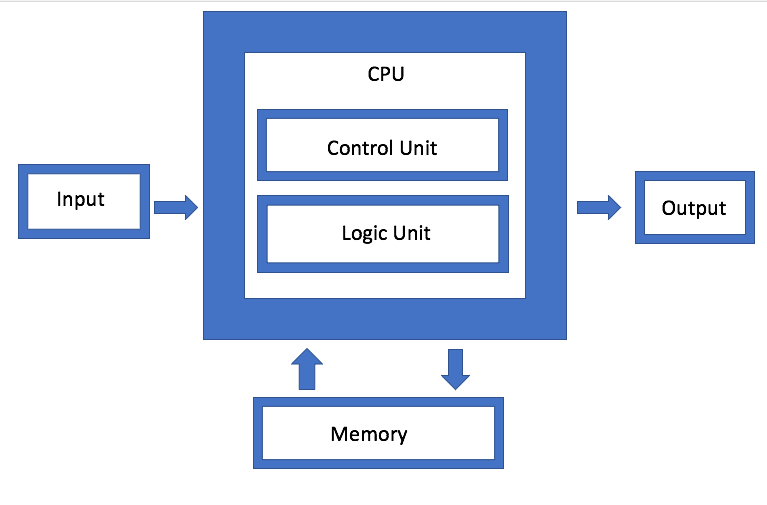
\includegraphics[width=0.9\linewidth]{./figures/sd_sc_code/neuman_en.png}
\end{figure}
\end{frame}

\begin{frame}{\\Von Neumann Architecture}
\topline
\justifying
\large
\begin{textitemize}
\item computer memory is homogeneous (linear)
\item access to computer memory cells is carried out at the address
\item alphabet used to represent data and commands is the set \{0, 1\}
\item each program consists of a set of instructions executed by the processor sequentially
\item conditional jump commands may be present in programs
\end{textitemize}
\end{frame}

\begin{frame}{\\Binary representation}
\topline
\justifying
\begin{columns}[T,onlytextwidth]
\begin{column}{0.6\textwidth}
	\vspace{10mm}
	\begin{figure}[H]
		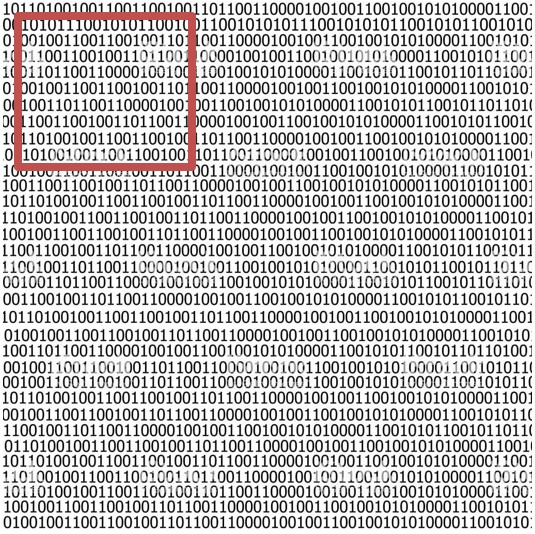
\includegraphics[scale=0.5]{./figures/sd_sc_code/binary.jpg}
	\end{figure}		
\end{column}

\begin{column}{0.4\textwidth}
	\vspace{10mm}
	\textbf{Advantages:}
	\begin{textitemize}		
		\item is easy to implement
		\item convenient for the computer
	\end{textitemize}		
	
	\bigskip
	\textbf{Disadvantages:}
	
	\begin{textitemize}		
		\item is inconvenient for a human
		\item cannot be interpreted without context
	\end{textitemize}	
	
\end{column}
\end{columns}
\end{frame}

\begin{frame}{\\Proposed approach}
\topline
\justifying
\large
Develop a method of encoding information that

\begin{textitemize}
\item is convenient for presentation and processing on a computer
\item is easy for human perception
\item has "meaningfulness"{}, can be interpreted unambiguously		
\end{textitemize}

\bigskip
A transition from \textit{data} to \textit{knowledge} is required.

\bigskip
One of the key distinguishing features of knowledge is interpretability (D. A. Pospelov).

\end{frame}

\begin{frame}{\\SC-code}
\topline
\justifying
\begin{SCn}
\scnheader{SC-code}
\scnidtf{a method of universal semantic representation (coding) of information in the memory of computer systems}
\scnidtf{semantic computer code}
\scntext{note}{SC-code is based on \underline{graph theory} (syntax) and \underline{set theory} (semantics), which ensures universality and unification (uniformity) of information presentation, ease of machine processing and human perception}
\end{SCn}
\end{frame}

\begin{frame}{\\Comparison of SC-code and binary coding}
\topline
\justifying
\vspace{10mm}
\begin{textitemize}
\item \textbf{Binary encoding}
\begin{textitemize}
	\item alphabet \{0, 1\}
	\item not convenient for humans
	\item computer-friendly
	\item information cannot be understood without context
	\item easy to implement
\end{textitemize}
\item \textbf{\textit{SC-code}}
\begin{textitemize}
	\item the basic alphabet consists of 5 elements
	\item human-friendly
	\item computer-friendly
	\item has "meaningfulness"{}
\end{textitemize}
\end{textitemize}
\end{frame}

\begin{frame}{\\Forms of SC-code representation}
\topline
\justifying
\vspace{10mm}
\begin{SCn}
\scnheader{SC-code}
\scnidtf{an abstract language that is stored in the memory of a computer system}
\scntext{note}{SC-code can be used to describe knowledge bases, problem solvers, and the interface of an intelligent system. SC-code is an abstract language, but it can be visualized in various forms.}
\vspace{5mm}
\textbf{Forms of external representation of SC-code}
\begin{textitemize}
	\item {SCs-code (text linear)}
	\item {SCn code (hypertext)}
	\item {SCg-code (graphic)}
\end{textitemize}
\end{SCn}
\end{frame}

\begin{frame}{\\Forms of SC-code representation}
\topline
\justifying
\vspace{5mm}
\begin{columns}[T,onlytextwidth]
\begin{column}{0.4\textwidth}
	\begin{SCn}
		\scnheader{SCs}
		\scnidtf{Semantic Code string}
		\scnidtf{linear knowledge representation language}
		\scnheader{SCn}
		\scnidtf{Semantic Code natural}
		\scnidtf{structured knowledge representation language}
		\scnheader{SCg}
		\scnidtf{Semantic Code graphic}
		\scnidtf{language of graphical representation of knowledge}
	\end{SCn}
\end{column}
\begin{column}{0.5\textwidth}
	\vspace{10mm}
	\begin{figure}[H]
		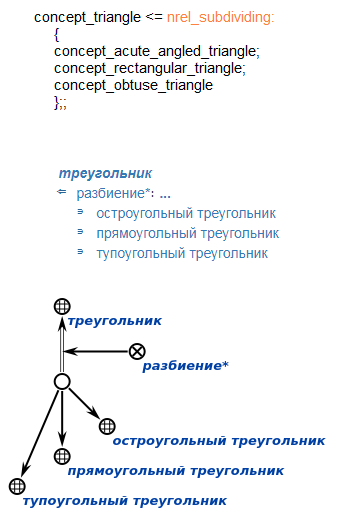
\includegraphics[scale=0.37]{./figures/sd_sc_code/ostis-basics-1.png}
	\end{figure}
\end{column}
\end{columns}
\end{frame}

\begin{frame}{\\Basic Principles of SC-code}
\topline
\justifying
\vspace{8mm}
\begin{SCn}
\scnheader{SC-code}
\scntext{explanation}{The information is contained not in the signs themselves, but in the configuration of connections between them}
\scniselement{abstract language}
\scniselement{graph language}
\begin{scnrelfromset}{basic principles}
	\scnfileitem{entity signs are syntactically elementary fragments of sc-texts; such signs have no internal structure}
	\scnfileitem{information constructs that are not sc-texts (SC-code texts) can be included in the knowledge base as files}
	\scnfileitem{SC-code texts have a nonlinear structure, since each entity sign is included in the knowledge base only once and has an unlimited number of connections with other entity signs}
\end{scnrelfromset}
\end{SCn}
\end{frame}

\begin{frame}{\\}
\topline
\justifying
\begin{SCn}
\scnheader{SC-code}
\begin{scnrelfromset}{basic principles}
	\scnfileitem{a knowledge base is a graph structure whose element alphabet includes a set of nodes, edges, arcs, base arcs, and a set of special nodes (files)}
	\scnfileitem{The structural feature of the graph structure of a knowledge base is that its arcs and edges can connect not only node to node, but also node to edge or arc, etc.}
	\scnfileitem{the absence of synonymy is achieved by gluing together identical sc-elements}
	\scnfileitem{sc-nodes, sc-edges, and sc-arcs are designations of different entities}
\end{scnrelfromset}
\end{SCn}
\end{frame}

\begin{frame}{\\Syntax. SC-code alphabet}
\topline
\justifying
\begin{SCn}
\scnheader{SC-code alphabet}
\scnidtf{a family of syntactic labels assigned to sc-elements and indicating the fact that the sc-element belongs to the corresponding class of sc-elements}

\scnheader{minimum SC-code alphabet}
\scntext{explanation}{To understand sc-constructions stored in sc-memory, it is sufficient to syntactically extract only the \textit{Class of constant positive sc-membership pairs (Class of basic sc-arcs)}, through which each sc-element will be explicitly connected to the sc-classes to which this sc-element belongs. Obviously, it is impossible to extract basic sc-arcs in such an explicit way using these basic sc-arcs themselves.}
\end{SCn}
\end{frame}

\begin{frame}{\\Minimal alphabet of the SC-code}
\topline
\justifying
\begin{SCn}
Thus, any class of sc-elements can be identified explicitly by:\\
\begin{textitemize}
	\item{introduction of an sc-element, which is a sign of this class of sc-elements (sc-class);}
	\item{setting of constant positive sc-pairs of membership into all sc-elements that are elements of mentioned sc-class and stored (present) in the current state of sc-memory.}
\end{textitemize}

\scnheader{minimum SC-code alphabet}
\scnidtf{\textit{Class of base sc-arcs} and \textit{Class of all other sc-elements} (default)}
\end{SCn}
\end{frame}

\begin{frame}{\\SC-code Core Alphabet}
\topline
\justifying
\begin{SCn}
\begin{columns}[T,onlytextwidth]
	\begin{column}{0.7\textwidth}
		\vspace{5mm}
		\scnheader{SC-code Core Alphabet}
		\begin{scneqtoset}
			\scnitem{sc-node, which is a file sign}
			\scnitem{sc-node, which is not a file sign}
			\scnitem{basic sc-arc}
			\scnitem{sc-edge}
			\scnitem{sc-arc of general type}
		\end{scneqtoset}
	\end{column}
	\begin{column}{0.3\textwidth}
		\begin{figure}[H]
			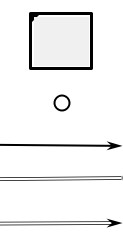
\includegraphics[scale=0.7]{./figures/sd_sc_code/abc.png}
		\end{figure}
	\end{column}
\end{columns}
\end{SCn}
\end{frame}

\begin{frame}{\\SC-code Core Alphabet}
\topline
\justifying
\begin{SCn}
\vspace{10mm}

\scriptsize

\scnheader{sc-edge}
\scnidtf{Class of \textit{sc-elements} that have, within the \textit{Core of SC-code}, the syntactic label \textit{designations of undirected sc-pairs}}

\scnheader{sc-arc of general type}
\scnidtf{Class of \textit{sc-elements} that have, within the \textit{Core of SC-code}, the syntactic label \textit{designations of oriented sc-pairs that are not constant positive sc-pairs of membership}}

\scnheader{basic sc-arc}
\scnidtf{Class of \textit{sc-elements} that have, within the framework of the \textit{Core SC-code}, the syntactic label \textit{constant positive sc-membership pairs}}

\scnheader{sc-node, which is the file sign}
\scnidtf{\textit{sc-elements}, which has within the \textit{SC-code core} the syntactic label \textit{sc-elements}, which are signs of \textit{files}}

\scnheader{sc-node, which is not a file sign}
\scnidtf{\textit{sc-node}, which has within the \textit{SC-code core} the syntactic label \textit{sc-elements that are neither file signs nor designations of sc-pairs}}
\end{SCn}
\end{frame}

\begin{frame}{\\Semantic classification of sc-elements}
\topline
\justifying
\textbf{}\\
The basic classification features of \textit{sc-elements} include:
\begin{textitemize}
\item structural feature;
\item logical-semantic feature;
\item temporal characteristic of entities designated by sc-elements, which in turn includes:
\begin{textitemize}
	\item permanence or temporariness of the existence of the designated entity;
	\item staticity (stationarity) or dynamism (variability) of the designated entity.
\end{textitemize}
\end{textitemize}
\end{frame}

\begin{frame}{\\Structural classification of sc-elements}
\topline
\justifying
\vspace{10mm}
\begin{SCn}
\scnheader{sc-element}
\scnrelfrom{subdividing}{Structural feature of classification of sc-elements}
\begin{scnindent}
	\begin{scneqtoset}
		\scnitem{sc-set designation}
		\scnitem{external entity designation}
		\begin{scnindent}
			\begin{scnrelfromset}{subdividing}
				\scnitem{file designation}
				\scnitem{designation of an information construct that is neither an sc-set nor a file}
				\scnitem{designation of an external entity that is not an information construct}
			\end{scnrelfromset}
		\end{scnindent}
	\end{scneqtoset}
\end{scnindent}
\end{SCn}
\end{frame}

\begin{frame}{\\Structural classification of sc-elements}
\topline
\justifying
\vspace{3mm}
\footnotesize
\begin{SCn}
\scnheader{sc-set notation}
\begin{scnrelfromset}{subdividing}
	\scnitem{sc-connection notation}
	\begin{scnindent}
		\begin{scnrelfromset}{subdividing}
			\scnitem{sc-singleton designation}
			\scnitem{sc-pair notation}
			\begin{scnindent}
				\begin{scnrelfromset}{subdividing}
					\scnitem{unoriented sc-pair designation}
					\scnitem{oriented sc-pair designation}
				\end{scnrelfromset}
			\end{scnindent}
			\scnitem{designation of an sc-connection that is neither a singleton nor a pair}
		\end{scnrelfromset}
	\end{scnindent}
	\scnitem{sc-class designation}
	\scnitem{sc-structure designation}
\end{scnrelfromset}
\end{SCn}
\end{frame}

\begin{frame}{\\}
\topline
\justifying
\begin{SCn}
\scnheader{oriented sc-pair designation}
\begin{scnrelfromset}{subdividing}
	\scnitem{designation of the sc-pair of membership}
	\begin{scnindent}
		\begin{scnrelfromset}{subdividing}
			\scnitem{designation of an sc-pair of fuzzy membership }
			\scnitem{designation of an sc-pair of positive membership}
			\scnitem{designation of an sc-pair of negative membership}
		\end{scnrelfromset}
	\end{scnindent}
	\scnitem{denotation of an oriented sc-pair that is not a membership pair}
\end{scnrelfromset}
\end{SCn}
\end{frame}

\begin{frame}{\\Logical-semantic classification}
\topline
\justifying
\begin{SCn}
\scnheader{Logical-semantic classification of sc-elements}
\scnstartstruct
\scnheader{sc-element}
\begin{scnrelfromset}{subdividing}
	\scnitem{sc-constant}
	\begin{scnindent}
		\scnidtf{sc-element, the logical-semantic meaning of which is itself}
	\end{scnindent}
	\scnitem{sc-variable}
\end{scnrelfromset}	
\scnendstruct
\end{SCn}
\end{frame}

\begin{frame}{\\}%Possibly unnecessary
\topline
\justifying
\begin{SCn}
\scnheader{Classification of sc-elements by the temporal characteristics of the entities they denote}
\scnstartstruct
\scnheader{sc-element}
\scnrelfrom{subdividing}{A sign of the constant existence of entities designated by sc-elements}
\begin{scnindent}
	\begin{scneqtoset}
		\scnitem{permanent entity designation}
		\begin{scnindent}
			\scnidtf{designation of a permanently existing entity}
		\end{scnindent}
		\scnitem{temporary entity designation}
	\end{scneqtoset}
\end{scnindent}
\scnendstruct
\end{SCn}
\end{frame}

\begin{frame}{\\Static entity indicator}%Possibly redundant
\topline
\justifying
\begin{SCn}
\scnheader{sc-element}
\scnrelfrom{subdividing}{Staticity indicator for entities denoted by sc-elements}
\begin{scnindent}
	\begin{scneqtoset}
		\scnitem{static entity designation}
		\begin{scnindent}
			\scnidtf{designation of an entity, changes to which within the relevant period of time are considered insignificant}
			\scnsuperset{notation for a static sc-set}
		\end{scnindent}
		\scnitem{dynamic entity designation}
		\begin{scnindent}
			\scnidtf{designation of an entity changing over time}
			\scnsuperset{notation for a dynamic sc-set}
		\end{scnindent}
	\end{scneqtoset}
\end{scnindent}
\end{SCn}
\end{frame}

\begin{frame}{\\Designation of a temporary entity}%Possibly redundant
\topline
\justifying
\begin{SCn}
\scnheader{temporary entity designation}
\begin{scnrelfromset}{subdividing}
	\scnitem{designation of an external temporal entity}
	\begin{scnindent}
		\scnsuperset{external situation designation}
		\scnsuperset{external event designation}
		\scnsuperset{external process designation}
	\end{scnindent}
	\scnitem{designation of an internal temporary entity in sc-memory}
\end{scnrelfromset}
\end{SCn}
\end{frame}

\begin{frame}{\\}%Possibly unnecessary
\topline
\justifying
\begin{SCn}
\scnheader{designation of an internal temporary entity in sc-memory}
\begin{scnrelfromset}{subdividing}
	\scnitem{designation of a situation in sc-memory}
	\begin{scnindent}
		\scnidtf{designation of a situation that has arisen or is arising during the processing of information in sc-memory}
	\end{scnindent}
	\scnitem{designation of an event in sc-memory}
	\begin{scnindent}
		\scnidtf{designation of an event that has occurred or will occur during the processing of information in sc-memory}
	\end{scnindent}
	\scnitem{designation of an information process in sc-memory}
	\begin{scnindent}
		\scnidtf{designation of an internal process in sc-memory that is, has been, or will be occurring}
	\end{scnindent}
\end{scnrelfromset}
\end{SCn}
\end{frame}

\begin{frame}{\\Temporal properties of sc-elements}%Possibly redundant
\topline
\justifying
\vspace{10mm}
\begin{SCn}
\textbf{When talking about the temporal properties of sc-elements, we should clearly distinguish:}
\begin{textitemize}
	\item temporary nature of the presence of any sc-element in the knowledge base in which it is located
	\item temporary nature of the presence in sc-memory of the entire given sc-construction (situation in sc-memory);
	\item temporary nature of the existence of the external entity that the sc-element denotes;
	\item static (dynamic) nature of an external entity, designated by an sc-element; the dynamic nature of an external entity presupposes the presence in the sc-memory of a description of the process of changing the state or configuration of the specified external entity;
	\item dynamic sc-set, which is a reflection of the corresponding external process;
	\item dynamic sc-set, which is a reflection of the corresponding internal process
\end{textitemize}
\end{SCn}
\end{frame}

\begin{frame}{\\Structural classification of sc-constants}
\topline
\justifying
\begin{SCn}
This classification is completely analogous to the \textit{Structural classification of sc-elements}, in contrast to which it describes the structural classification of only constant sc-elements (sc-constants)
\end{SCn}
\end{frame}

\begin{frame}{\\Structural classification of sc-constants}
\topline
\justifying
\begin{SCn}
\scnheader{Structural classification of sc constants}
\scnstartstruct
\scnheader{sc-constant}
\begin{scnrelfromset}{subdividing}
	\scnitem{sc-set}
	\scnitem{external entity}
\end{scnrelfromset}

\scnendstruct
\end{SCn}
\end{frame}

\begin{frame}{\\external entity}
\topline
\justifying
\begin{SCn}
\scnheader{external entity}
\scnidtf{sc-element, which is a sign of an external entity}
\scnidtf{external entity sign}
\scnidtf{sign of an entity that is not an sc-set (sc-construction)}
\begin{scnrelfromset}{subdividing}
	\scnitem{file}
	\scnitem{internal file}
	\scnitem{external entity that is not an internal file}
	\scnitem{external entity that is not an information construct}
	\scnitem{information construct that is neither an sc-set nor a file}
\end{scnrelfromset}
\end{SCn}
\end{frame}

\begin{frame}{\\sc-set}
\topline
\justifying
\begin{SCn}
\scnheader{sc-set}
\begin{scnindent}
	\begin{scnrelfromset}{subdividing}
		\scnitem{sc-link}
		\begin{scnindent}
			\begin{scnrelfromset}{subdividing}
				\scnitem{sc-singleton}
				\scnitem{sc-pair}
				\scnitem{sc-connection that is neither a singleton nor a pair}
			\end{scnrelfromset}
		\end{scnindent}
		\scnitem{sc-class}
		\scnitem{sc-structure}
	\end{scnrelfromset}
\end{scnindent}
\end{SCn}
\end{frame}

\begin{frame}{\\sc-pair}
\topline
\justifying
\vspace{5mm}
\begin{SCn}
\scnheader{sc-pair}
\begin{scnrelfromset}{subdividing}
	\scnitem{unoriented sc-pair}
	\scnitem{oriented sc-pair}
	\begin{scnindent}
		\begin{scnrelfromset}{subdividing}
			\scnitem{sc-pair of membership}
			\begin{scnindent}
				\begin{scnrelfromset}{subdividing}
					\scnitem{sc-pair of fuzzy membership}
					\scnitem{sc-pair of positive membership}
					\scnitem{sc-pair of negative membership}
				\end{scnrelfromset}
			\end{scnindent}
			\scnitem{oriented sc-pair that is not a membership sc-pair}	
		\end{scnrelfromset}
	\end{scnindent}
\end{scnrelfromset}
\end{SCn}
\end{frame}

\begin{frame}{\\sc-pair of positive membership}
\topline
\justifying
\vspace{5mm}
\begin{SCn}
\scnheader{sc-pair of positive membership}
\scnsuperset{sc-pair of constant positive membership}
\begin{scnindent}
	\begin{scnreltoset}{intersection of sets}
		\scnitem{sc-constant}
		\scnitem{permanent entity}
		\scnitem{static entity}
		\scnitem{sc-pair of positive membership}	
	\end{scnreltoset}
\end{scnindent}
\scnsuperset{sc-pair of temporal positive membership}
\begin{scnindent}
	\begin{scnreltoset}{intersection of sets}
		\scnitem{sc-constant}
		\scnitem{temporary entity}
		\scnitem{dynamic entity}
		\scnitem{sc-pair of positive membership}	
	\end{scnreltoset}
\end{scnindent}
\end{SCn}
\end{frame}